%*****************************************
\chapter{Grundlagen}\label{ch:preliminaries}
%*****************************************
% \section*{Inhalte des Kapitels}
% - Taxonomie von Ammus (\citet{ammus}) % DONE
% - Transformer Architektur (\citet{attention}) % DONE

% - Neuronales Netz (https://katalog.ub.uni-leipzig.de/Record/0-1066754535) % DONE
% - Activation Functions (https://katalog.ub.uni-leipzig.de/Record/0-1066754535) % DONE
% - Backpropagation (https://katalog.ub.uni-leipzig.de/Record/0-1066754535)% DONE
% - Training eines Modells % DONE
%     - Batching % DONE
%     - Optimizer % DONE
%     - Learning Rate % DONE

% - Feed-Forward Netze
% - Multi-Head Attention
% - Encoder und Decoder

% - Input embeddings = Embeddings
% - Positional Embeddings
% - Tokenization % DONE
%     - Byte Pair Encoding % DONE


% Sprachmodell Definition (Was ist das)

% - Autoregressive Modelle % DONE
%     - Self-supervised Learning % DONE
%     - Pretraining
%     - continual Pretraining
%     - Decoder-Based % DONE
%     - ZeroShot / FewShot

% - Weiterentwicklungen
%     - Deep Residual Connections % DONE
%     - DropOut   % DONE

% Wissen, Information, Daten (Winter)
% FScore, Precision, Recall, Micro und MacroF1 (QUALD9)
% Question Answering (Aggregation, erst FScore für Frage, dann Durchschnitt, oder andersrum)
% API, Overfitting
%************ Sprachmodelle
Um die genannten Ziele aus \cref{sec:zielsetzung} lösen zu können und den Lösungsschritten in \cref{ch:approach} zu folgen, werden in diesem Kapitel Grundlagen gelegt für Begriffe und Konzepte, die in dieser Arbeit verwendet werden.
Das Kapitel teilt sich auf in einer generellen Begriffserklärung zu Sprachmodellen in \cref{sec:sprachmodelle} mit einer genaueren Erklärung zu der Transformer-spezifischen Architektur.
Anschließend wird ein kurzer Einstieg in das Thema Neuronale Netze gegeben, in der die Funktionsweise dieser genauer betrachtet wird \pcref{sec:neuronale-netze}.
Zuletzt finden sich noch einige Begriffserklärungen aus der Medizininformatik und der Davenverarbeitung in \cref{sec:datenverarbeitung}.

\section{Sprachmodelle}\label{sec:sprachmodelle}

\begin{definition}\label{def:sprachmodell}
   \textbf{Sprachmodelle} sind computergestützte Systeme, welche menschliche Sprache  verstehen und darauf reagieren.
\end{definition}
Sprachmodelle basieren auf künstlicher Intelligenz und werden in der Regel durch maschinelles Lernen trainiert.
Sprachmodelle finden in einer Vielzahl an Anwendungen ihren Einsatz, wie zum Beispiel in der Übersetzung,
Textgenerierung, Spracherkennung, Chatbots und Textklassifizierung.

\begin{definition}\label{def:autoregressive-sprachmodelle}
    \textbf{Autoregressive Sprachmodelle} sind eine Art von Sprachmodellen, die entwickelt wurden, um Texte zu generieren,
    indem sie die Wahrscheinlichkeit von Wörtern oder Zeichen in einer Sequenz vorhersagen.
\end{definition}

Autoregressive Modelle basieren auf der Annahme, dass jedes Element in der Sequenz abhängig von den vorherigen Elementen ist.
In einem Autoregressiven Sprachmodell wird die generative Wahrscheinlichkeit eines nächsten Elements in der Sequenz geschätzt.
Die Ausgabe im Kontext von Decoder-basierten Modellen ist demnach eine Wahrscheinlichkeitsverteilung über das mögliche nächste Element.
Das wahrscheinlichste Element wird dann der Sequenz hinzugefügt und der Prozess wird wiederholt, bis die Sequenz fertig ist.
Überlicherweise werde Autoregressive Sprachmodelle auf großen Textdatenmengen trainiert, um die statistischen Zusammenhänge in den Trainingsdaten zu erfassen.

\subsection{Transformer-Modelle}\label{sec:grundlagen:transformer}

\begin{definition}\label{def:transformer-modell}
    Ein \textbf{Transformer-Modell} ist ein Sprachmodell, das auf der Transformer-Architektur von \citet{attention} basiert.
\end{definition}
Im Gegensatz zu früheren Sprachmodelle, die auf rekurrenten oder faltenden neuronalen Netzen basieren, verwendet der Transformer ein Aufmerksamkeitsmechanismus (engl. Attentionmechanism), um Beziehungen zwischen Wörtern in einem Satz zu modellieren.
Transformer-Modelle bestehen aus einer Stapelung von Encoder- und Decoder-Schichten, wobei der Encoder zur Extraktion von Kontextinformationen aus der Eingabe dient,
während der Decoder die Ausgabe des Encoders verwendet, um die gewünschte Aufgabe zu lösen.
Die Architektur eines Transformers ist in \cref{bild:transformer} zu sehen.\\

\begin{figure}[ht]
    \centering
    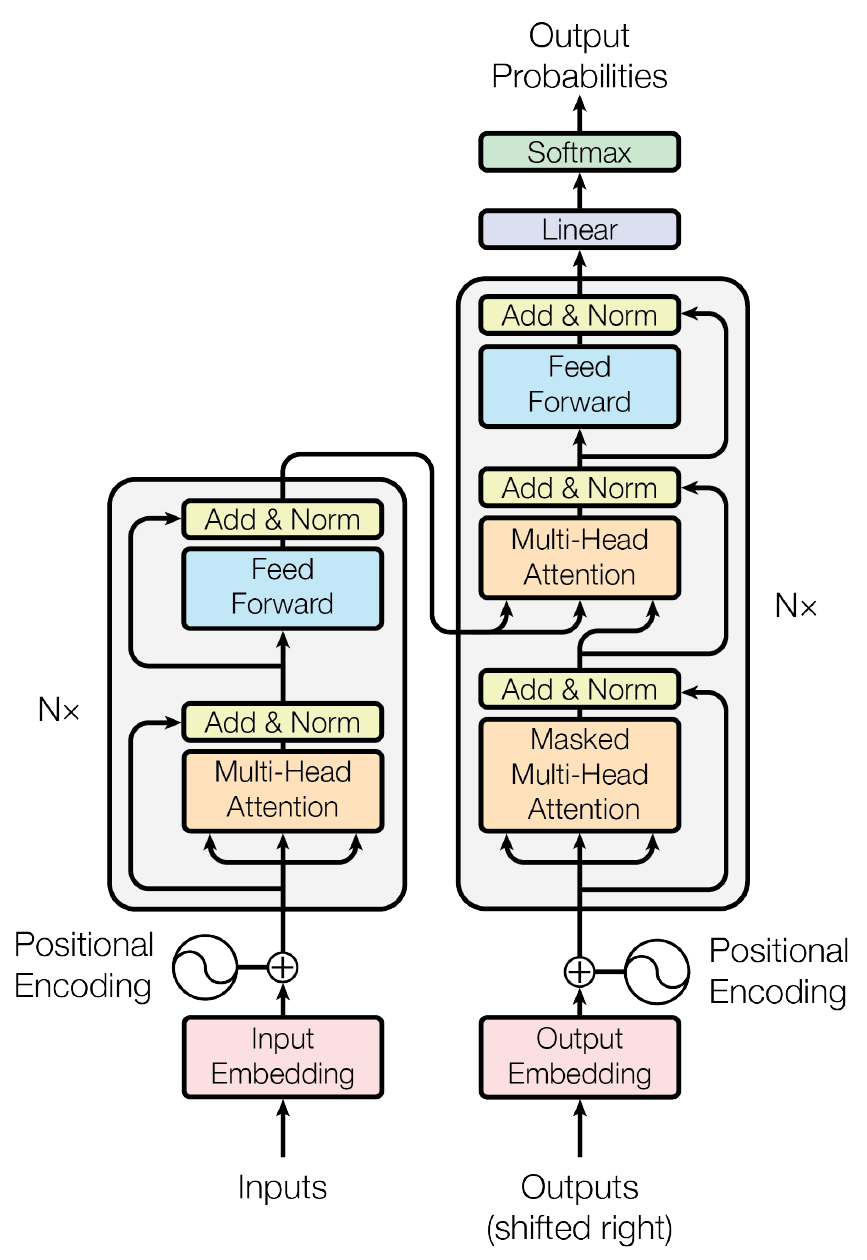
\includegraphics[width=0.8\textwidth]{zeichnungen/transformer.png}
    \caption{Die Transformer-Modell Architektur \citep{attention}}
    \label{bild:transformer}
\end{figure}

Die erste schriftliche Erwähnung des Transformer-Modells und zusätzlich auch die Einführung der beiden Teilmodelle Encoder und Decoder findet sich in \citet{attention}.
Die hier beschriebene bidirektionale Architektur bildet die Grundlage für alle darauf aufbauenden Modelle und Weiterentwicklungen.
Die grundlegende Architektur wurde für verschiedene Anwendungen stark modifiziert.
Seit 2017 gibt es grundlegende Unterschiede in den Modellen und deren Möglichkeiten.
Aus diesem Grund haben \citet{ammus} eine Taxonomie der Transformer-basierten vortrainierten Sprachmodelle eingeführt.
Diese Taxonomie wird hier zur Beschreibung weiterer Architekturen und Methodiken verwendet.\\

Neben dem Grundbaustein eines Transformers - dem Attention-\ac{nn} - sind zwei wichtige Modifikationen gegenüber normalen neuronalen Netzen in Transformer eingeflossen: Residuale Verbindungen und Dropout.\\

\subsubsection{Residuale Verbindungen}

\begin{definition}\label{def:residuale-verbindungen}
    \textbf{Residuale Verbindungen} oder auch Deep Residual Connections, sind direkte Verbindungen zwischen Eingabe und Ausgabe und überspringen somit eine oder mehrere Schichten eines \ac{nn}.
\end{definition}
Residuale Verbindungen als Level-Normalisierung verändern das Ziel eines \ac{nn}, behalten aber durch ihre Level-Normalisierung die gleichen Ausgaben bei.
Dieses Konzept wurde erstmals in \citet{deep_residual} eingeführt und liefert die Lösung für ein grundlegendes Problem von großen, aus mehreren Ebenen bestehenden Transformer-Modellen.
Bereits 2016 wurde im Bereich der Bilderkennung festgestellt, dass sich die Korrektheit von Modellen mit zunehmender Tiefe sättigt und dann schnell verschlechtert, wenn dieses Modell weiter trainiert wird.
Dies setzte eine praktische Grenze für die Tiefe von \ac{nn}s und verhinderte somit die Lösung komplexerer Probleme mit größeren Modellen.
\citet{deep_residual} beschreiben eine Lösung durch die genannten Residuen, die normale \ac{nn} simple ersetzen können, und zeigen ebenfalls die Wirksamkeit dieser Methode.\\

\subsubsection{Dropout}

Die zweite wichtige Änderung zur Weiterentwicklung der Transformer-Architektur ist die Einführung von Dropouts.
\begin{definition}\label{def:dropout}
    \textbf{Dropout} ist eine Methode, die die Trainingszeit von \ac{nn}s verkürzt und die Generalisierung verbessert.
    \citet{dropout} beschreiben die Methode als das zufällige Aussetzen von Neuronen unabhängig von der Eingabe in einem \ac{nn} während des Trainings. 
\end{definition}
Durch das Aussetzen von Neuronen wird das \ac{nn} gezwungen, sich nicht auf andere Neuronen zu verlassen und somit eine bessere Generalisierung zu erreichen.
Das Aussetzen erfolgt nur während des Trainings und nicht während der Inferenz.
Die Methode wurde 2014 eingeführt und ist seitdem ein fester Bestandteil von \ac{nn}s.\\

\subsubsection{Modellarten von Transformer-Modellen}

Auf Basis der eingeführten Transformer-Architektur wurden verschiedene Modellarten entwickelt, welche nur Teile der Architektur verwenden und sich in ihrer Funktionsweise unterscheiden.

\begin{definition}\label{def:encoder-basierte-modelle}
    \textbf{Encoder-basierte Modelle} sind Sprachmodelle, die hauptsächlich auf der Encoder-Architektur basieren.
    Sie wurden entwickel, um Eingabesequenzen zu verarbeiten und eine kompakte Repräsentation (auch Kontextvektor genannt) zu erstellen.
\end{definition}
Ein zentrale Komponente eines Encoder-basierten Modells ist der Encoder.
Er nimmt die Eingabesequenz entgegen und lernt schrittweise die strukturellen und semantischen Informationen zu erfassen.
Die erzeugte Repräsentation des Encoders kann von anderen Modulen oder Schichten des Modells zur Lösung von verschiedenen Aufgaben 
wie zum Beispiel der Klassifikation verwendet werden.
Encoder-basierte Modelle besitzen in der Regel keine Decoder-Schichten.\\

\begin{definition}\label{def:decoder-basierte-modelle}
    \textbf{Decoder-basierte Modelle} sind Sprachmodelle, die auf einer speziellen Architektur basieren, bei der der Decoder eine zentrale Rolle spielt.
    Der Decoder ist eine Komponente, die darauf spezialisiert ist aus einer gegebenen Eingabe eine sinvolle und zusammenhängende Ausgabe zu generieren.
\end{definition}
Im Kontext der Textgenerierung erhält der Decoder in der Regel eine Sequenz von Vektoren als Eingabe, die von einem Encoder-Modul erstellt wurden.
Bei der Textgenerierung kann der Decoder auf einer gegebenen Anfangssequenz fortlaufend neue Wörter oder Sätze generieren, um einen zusammenhängenden Text zu erzeugen.

\subsection{Transformer-spezifische Architekturen}

\begin{definition}\label{def:self-attention-mechanismus}
    Der \textbf{Self-Attention-Mechanismus} ist ein zentrales Konzept in der Transformer-Architektur und beschreibt die Gewichtung der Eingabesequenz auf Basis eines aktuellen Tokens.
\end{definition}
Hier wird ein Eingabevektor in drei separate Vektoren transformiert:
den Abfragenvektor (engl. Query), den Schlüsselvektor (engl. Key) und den Wertvektor (engl. Value).
Anschließend wird die Ähnlichkeit zwischen Abfragevektor und Schlüsselvektor berechnet,
um die Aufmerksamkeitsgewichte zu erhalten.
Die Aufmerksamkeitsgewichte geben an, wie wichtig jeder Wertvektor für die Berechnung eines gewichteten
Durchschnitts ist. Die gewichteten Wertvektoren werden schließlich summiert, um den Ausgabevektor zu erhalten.
Self-Attention-Mechanismen ermöglichen es Modellen, komplexe Abhängigkeiten zwischen den Element einer Eingabesequenz zu erfassen.\\

\begin{definition}\label{def:multi-head-attention}
    \textbf{Multi-Head Attention} beschreibt den Ersatz eines einzelnen Self-Attention-Mechanismus in der Transformer-Architektur durch mehrere Self-Attention-Mechanismen in parallel.
\end{definition}
Bei dem Prozess es Multi-Head Attention werden Abfrage, Schlüssel und Wert linear $h$ mal auf mehrere Versionen projeziert und parallel berechnet. Die Ausgabe wird daraufhin konkateniert und erneut linear projeziert, um den Ausgabevektor zu erhalten. Multi-Head Attention ermöglicht es dem Modell, verschiedene Repräsentation-Subspaces der Eingabe an unterschiedlichen Positionen zu erfassen.

\begin{definition}\label{def:feed-forward-netz}
    Ein \textbf{Feed-Foward-Netz} ist eine Art von künstlichem neuronalem Netz, welches aus mehreren Schichten bestehend Information ausschließlich vorwärts von der Eingabe
    in Richtung der Ausgabe fließen lässt.
\end{definition}
Feed-Foward-Netz besitzen keine zyklischen Verbindungen oder Rückkopplungsschleifen.
Sie dienen in Transformern neben Attention-Netzen als einzige zweite Komponente der Architektur.
Sie enthalten das erlernte Faktenwissen des Modells durch so genannte Wissensneuronen \citep{knowledge_neurons}.\\

\subsection{Eigenheiten von Transformer-Modellen}
\begin{definition}\label{def:zeroshot-oneshot-multishot}
    Die Bezeichnungen \textbf{ZeroShot, OneShot} und \textbf{MultiShot} beziehen sich auf die Inferenz von Modellen.
    Die Eingabe enthält hierbei Aufgabenbeispiele, bevor die eigentliche Aufgabe gestellt wird.
\end{definition}
Gerade bei \ac{qa}-Aufgaben und Text-Generierungen kommen häufig diese Methoden zu Anwendung.
Bei der Beantwortung von Fragen können Eingaben mehrere Beispielfragen und deren Antworten enthalten, bevor die eigentliche Frage gestellt wird.
Dies führt dazu, dass das Modell aus dem Kontext die Formatierung und Art der Aufgabe erkennt und bessere Antworten liefern kann.
\mbox{ZeroShot} bedeutet, dass das Modell keine Trainingsbeispiele erhält, um eine bestimmte Aufgabe zu lösen.
OneShot bedeutet, dass das Modell nur ein Trainingsbeispiel erhält, um eine bestimmte Aufgabe zu lösen.
MultiShot bedeutet, dass das Modell mehrere Trainingsbeispiele erhält.


\begin{definition}\label{def:parameterformate}
    \textbf{Parameterformate} sind Variableneinheiten von lernbaren Parametern.
    Häufig benutzt sind hier \enquote{Float16} und \enquote{Float32}.
\end{definition}
Sprachmodelle enthalten eine große Anzahl an lernbaren Parametern (wie zum Beispiel Gewichte und Bias),
als auch Zwischenwerte, die während der Inferenz berechnet werden.
Diese Werte können in verschieden Formaten gespeichert werden.
Häufige Formate sind hier \enquote{Float16} und \enquote{Float32}.
Float steht hier für Floating Value und repräsentiert eine Gleitkommazahl.
Die Zahl hinter Float gibt die Anzahl der Bits an, die für die Darstellung der Zahl verwendet werden.
Eine höhere Bitzahl bedeutet eine höhere Genauigkeit, aber auch ein höherer Speicherbedarf.

\begin{definition}\label{def:continual-pretraining}
    \textbf{Continual Pretraining} beschreibt den Prozess des fortlaufenden selbstüberwachten Trainings eines vortrainieren Modells.
\end{definition}
Bei Continual Pretraining werden lediglich die Hyperparameter des Modells angepasst und neue Datensätze verwendet, während die erlernten Parameter des Modells beibehalten werden.

%************ Transformer-Spezifische Eingaben

\subsection{Eingaben von Transformer-Modellen}
\begin{definition}\label{def:token}
    Ein \textbf{Token} repräsentiert eine Teilmenge eines Wortes und wird in Transformer-Modellen verwendet, um die Eingabe in logische Einheiten zu unterteilen.
\end{definition}
Transformer-Modelle können Eingaben nicht ohne zusätzliche Umwandlung verarbeiten.
Neben der Erzeugung von Eingabevektoren muss die Eingabe zunächst in kleinere Einheiten, sogenannte Tokens, zerlegt werden.
Verschiedene ältere Modelle verwenden dazu Wörter oder Symbolunterteilungen.
Dies ist jedoch problematisch.\\

Durch die Zerlegung der Eingaben in Symbole ist zwar das Vokabular kleiner, welches zu schnelleren Trainingsdurchläufen führt, jedoch muss das Modell vor dem Erlernen von Wortzusammenhängen, Satzstrukturen und Sachverhalten zunächst die Bedeutung der Wörter und deren Zusammensetzung aus Symbolen erlernen.
Dies führt dazu, dass ein großer Teil der Trainingszeit für das Erlernen der Sprache verloren geht, was die endgültige Leistungsfähigkeit der Modelle massiv einschränkt \citep{bpe}.\\

\begin{definition}\label{def:vokabular}
    Das \textbf{Vokabular} eines Modells ist die Menge aller Tokens, die das Modell als einzelne Einheiten erkennt. Die Größe des Vokabluars bestimmt die Größe der Input Embeddings und limitiert damit die Größe der Eingaben.
\end{definition}

Eine logische Schlussfolgerung wäre hier die Verwendung von Wörtern oder sogar Satzphrasen als Tokens.
Mit zunehmender Größe der Datensätze, die zum Training der Modelle verwendet werden, wächst hier das Vokabular immens an.
Dies führt zu einer starken Verlangsamung der Trainingsläufe und zu sehr großen Modellen ohne Vorteil in ihrer Leistungsfähigkeit.
Wörter mit gleichem Wortstamm oder ähnlicher Bedeutung aufgrund grammatikalischer Regeln (Plural, Genus, Tempora) müssen vom Modell erst als \enquote{gleiches Wort} gelernt werden.
Daher hat sich die Unterteilung von Wörtern in Teilwörter als Standard durchgesetzt.

\subsubsection{Byte Pair Encoding}
\begin{definition}\label{def:bpe}
    \textbf{Byte Pair Encoding} ist ein Algorithmus, der iterativ ein Vokabluar aufbaut auf Basis der Häufigkeit von Symbolkombinationen in einem Datensatz.
    Die Vokabulargröße ist dabei der einzige Parameter.
\end{definition}
\citet{bpe} schlugen zu diesem Zweck die Verwendung von \ac{bpe} vor.
Die Unterteilung von Wörtern in Untergruppen von Wörtern hat bereits bei der Übersetzung von Sätzen zu erheblichen Verbesserungen geführt.
Sie hat sich aber auch in anderen Bereichen und Aufgaben wie der Textgenerierung, der Textklassifikation und der Analyse von Emotionen durchgesetzt.
Die Unterteilung von Wörtern ist hier eher als das Zusammenfügen kleinerer Teilwörter zu verstehen.
Ausgehend von einem Vokabular, das aus allen Symbolen eines Alphabets besteht, wird dieses durch das Zusammenführen (engl. \enquote{Merge}) von Symbolen erweitert, deren Kombination im Datensatz am häufigsten vorkommt.
Dieser Vorgang wird solange wiederholt, bis die gewünschte Anzahl von Teilwörtern erreicht ist.
Die Anzahl der Teilwörter ist dabei ein Hyperparameter, der je nach Modell und Datensatz variiert.\\

Die Unterteilung von Wörtern in Teilwörter hat den Vorteil, dass die Größe des Vokabulars nicht mit der Größe des Datensatzes wächst.
Dies führt zu einer schnelleren Eingabeverarbeitung und einer besseren Generalisierung der Modelle.
Die Unterteilung von Wörtern in Teilwörter hat jedoch auch Nachteile.
Sie ist nicht eindeutig, d.h. ein Wort kann in unterschiedliche Mengen von Teilwörtern zerlegt werden.
Dies führt zu einer größeren Anzahl möglicher Eingaben, die das Modell lernen muss.\\

Ein weiterer Nachteil ist, dass die Zerlegung von Wörtern in Teilwörter nicht immer sinnvoll ist.
So kann es vorkommen, dass ein Wort in Teilwörter zerlegt wird, die in der Sprache nicht existieren.
Dies wiederum minimiert die Verallgemeinerbarkeit der Modelle.
Ein Beispiel hierfür ist das Wort \enquote{Datensatz}.
Eine sinnvolle Unterteilung wäre hier \enquote{Daten} und \enquote{satz}, aber durch den Aufbau des Vokabulars aus den Symbolen des Datensatzes kann es vorkommen, dass das Teilwort \enquote{Daten} nicht die notwendige Häufigkeit besitzt und somit nicht im Vokabular vorhanden ist.
Daher muss auch dieses Wort zerlegt werden, z.B. in \enquote{Dat} und \enquote{en}.
Beide Teilwörter haben in der deutschen Sprache keine Bedeutung, werden aber durch das Modell mit Bedeutung belegt und in Beziehung zu anderen Wörtern gesetzt.
Dies führt zu einer unverständlichen Bedeutungsannotation von Teilwörtern und verschlechtert sowohl die Leistung als auch die Nachvollziehbarkeit des Modells und erschwert die Forschung an den Modellen.

\subsubsection{Eingabevektoren}

\begin{definition}\label{def:input-embeddings}
    \textbf{Input Embeddings} sind eine Darstellung der Eingabedaten wie Tokens in einem dichten Vektorraum.
\end{definition}
Die Darstellung von Tokens als Vektorraum muss erlernt werden und ermöglicht es,
Tokens die semantische Ähnlichkeiten aufweisen oder Beziehungen zueinander haben, geometrisch nahe beieinander zu platzieren.
Dadurch ist nicht nur der eigentliche Token bekannt, sondern auch die Beziehung zu anderen Tokens. Mit steigender Vokabulargröße muss ebenso die Dimensionen der Input Embeddings erhöht werden, da sonst ungewollte Kollisionen zwischen Tokens auftreten können.

\begin{definition}[Positional Encodings]\label{def:positional-encodings}
    \textbf{Positional Encodings} repräsentieren sogenannte relative und absolute Positionen der Tokens in der Eingabe.
\end{definition}
Relative und absolute Positionen von Tokens innerhalb einer Eingabe werden in einem Vektorraum dargestellt und erlauben es dem Modell, die Positionen der Tokens zu berücksichtigen.
Positional Encodings können erlernt oder berechnet werden und werden ausschließlich in Kombination mit Input Embeddings verwendet.

\section{Neuronale Netze}\label{sec:neuronale-netze}
Zum Verständnis der Transformer-Architektur ist es notwendig, die Grundlagen von Neuronalen Netzen zu verstehen.
Neuronale Netze wurden erstmalig 1943 von \citet{neuronal_networks_first} beschrieben und unterliefen seitdem vielen Veränderungen und Verbesserungen.
Eine Beschreibung grundlegender Techniken findet sich in \citet{neuronale-netze}.
Auf Basis dieses Buches wird in Folgendem ein Überblick über die Funktionsweise von Neuronalen Netzen gegeben.\\

\subsection{Architektur}
Neuronale Netze imitieren die Funktionsweise des menschlichen Gehirns mit Hilfe von mathematischen Gleichungen.
Ein Netz besteht aus einer Anzahl an Neuronen, welche sowohl Eingangs- als auch Ausgangsverbindungen zu anderen Neuronen besitzen.
Neuronen besitzen die Eigenschaft, aus gegebenen Eingängen einen Impuls zu den Ausgängen zu senden, wenn ein Schwellwert überschritten ist.
Anders als im Gehirn sind normale Neuronale Netze jedoch logischer aufgebaut.
Neuronen sind in Schichten angeordnet, wobei die erste Schicht die Eingabeschicht bestehend aus Eingabeneuronen $E_N$ und die letzte Schicht die Ausgabeschicht bestehend aus Ausgabeneuronen $A_N$ ist.
Schichten zwischen diesen beiden Grenzen nennt man Hidden Layers mit Neuronen $H^L_N$.\\

\begin{figure}
    \centering
    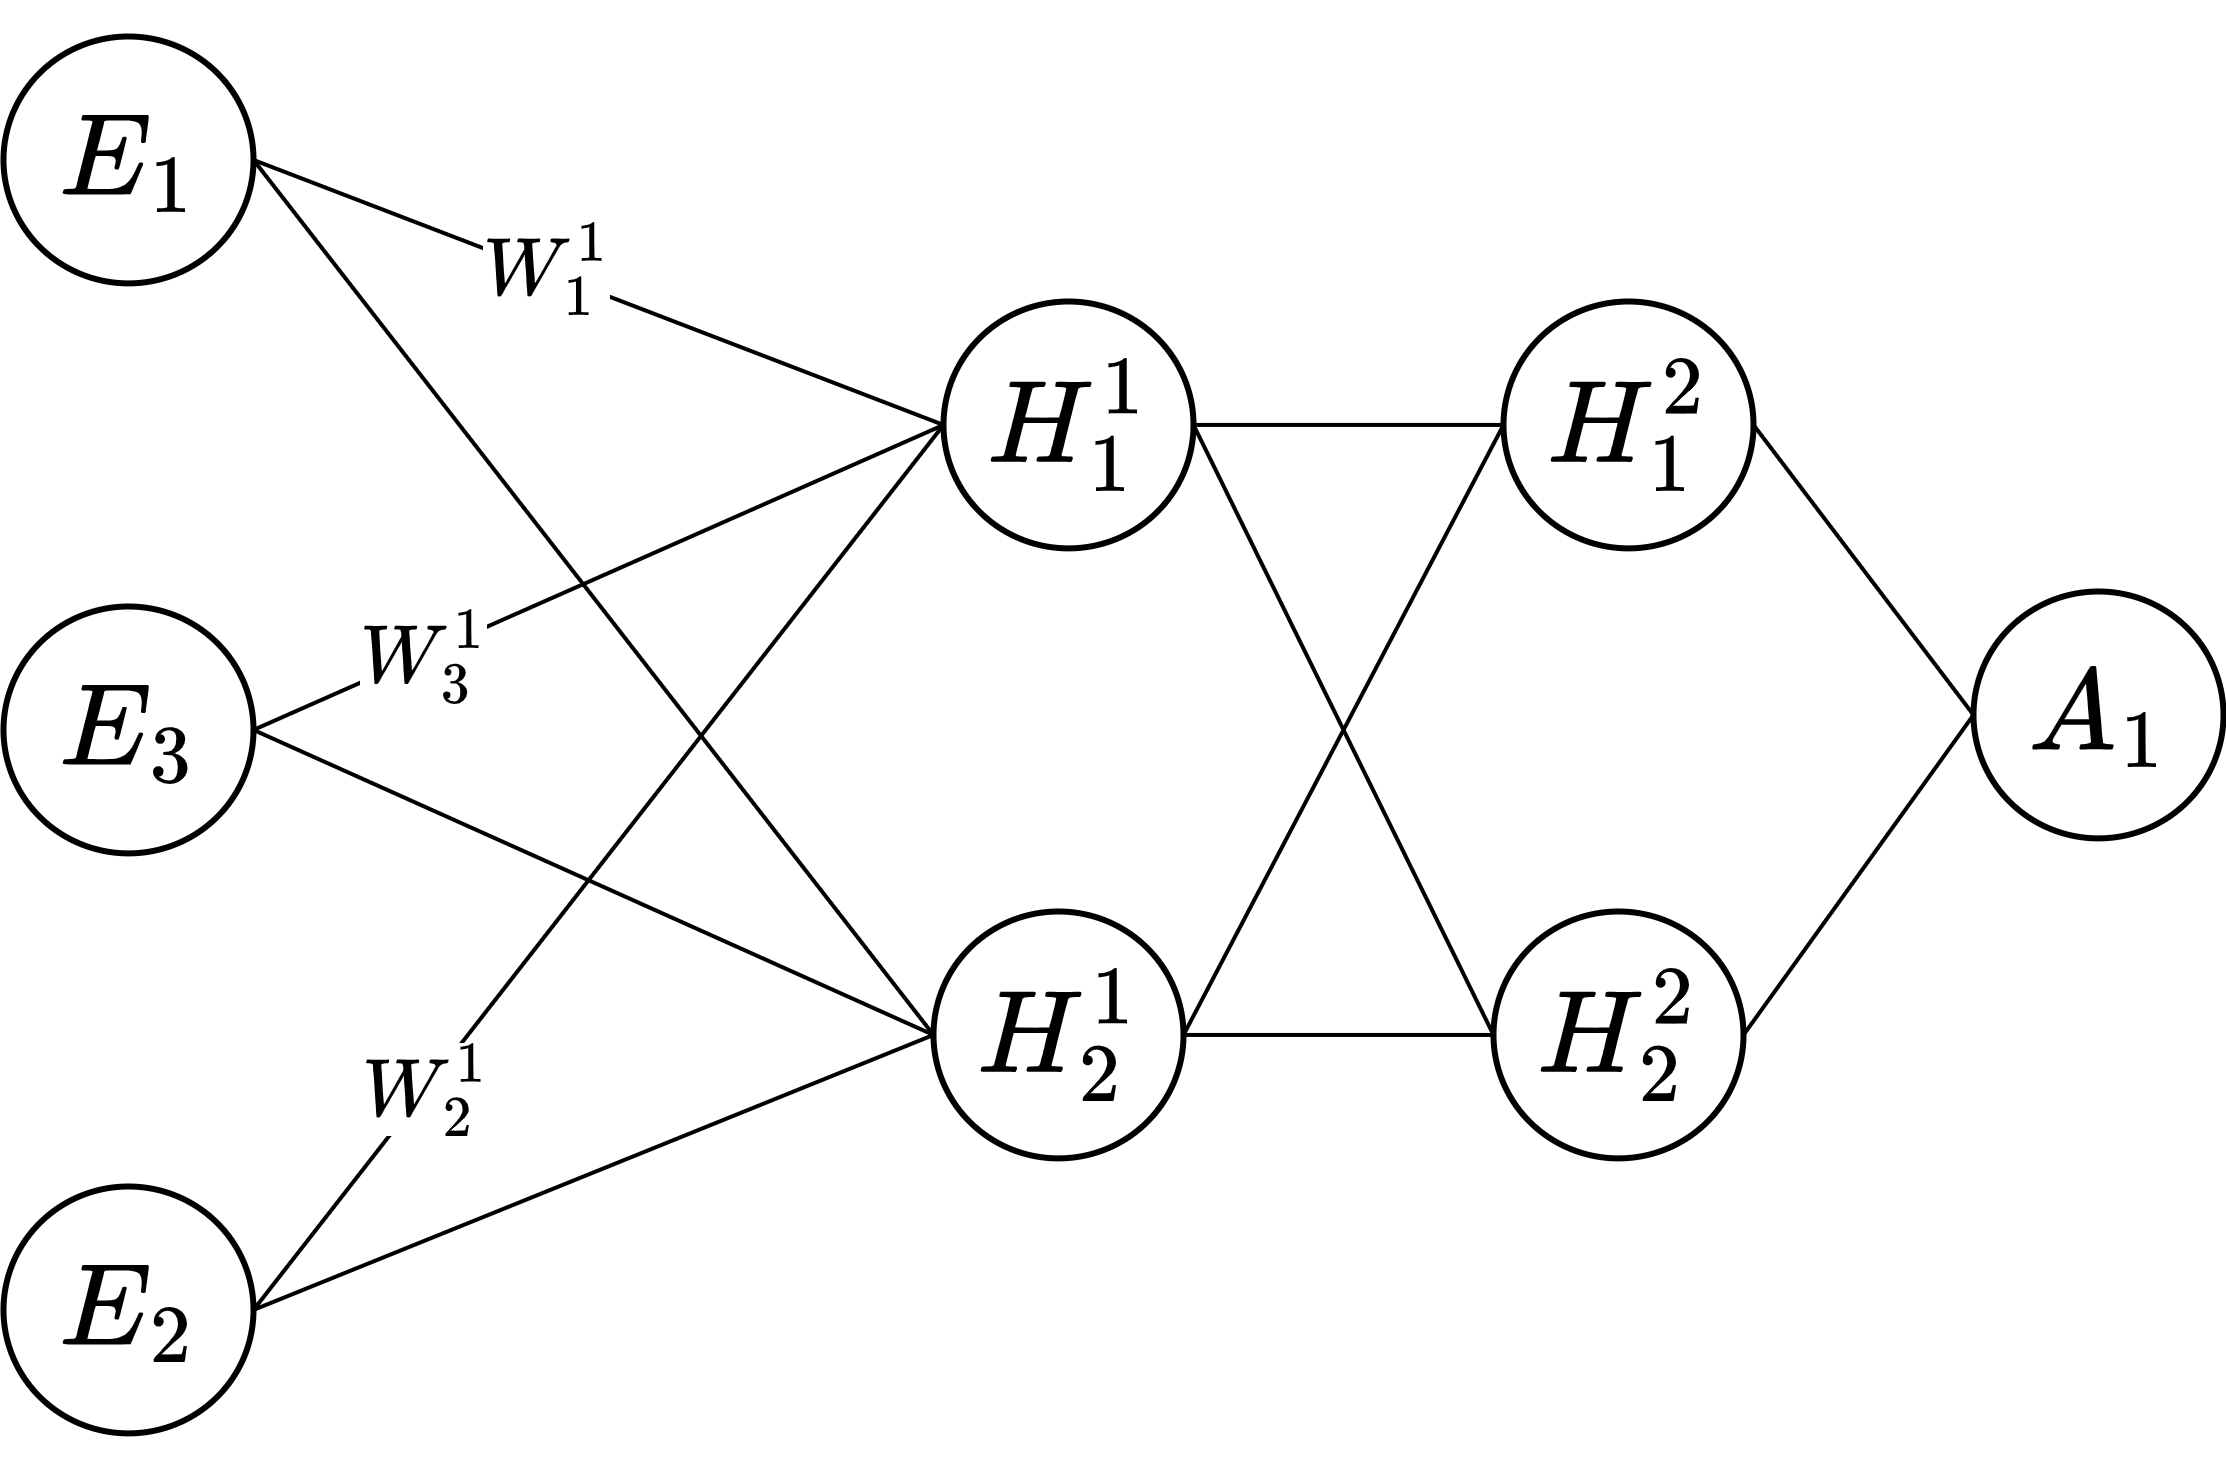
\includegraphics[width=\textwidth]{zeichnungen/nn.png}
    \caption{Beispiel-Aufbau eines Neuronalen Netzes mit 3 Eingabeneuronen, 4 Hidden Neuronen und einem Ausgabeneuron.}\label{nn_simple}
\end{figure}

\cref{nn_simple} zeigt einen Beispielaufbau mit 3 $E_N$, hier bezeichnet als $E_1,E_2,E_3$, zwei Hidden Layer mit je zwei $H^L_N$, hier bezeichnet als $H^1_1, H^1_2$ und $H^2_1, H^2_2$ und einem Ausgabeneuron $A_1$.
Verbunden sind Neuronen mit sogenannten Gewichten $W_N$. Man spricht hier von einer Vorwärts-Verbindung.
Dies bedeutet das Eingaben durch die Schichten in Richtung der Ausgabe weitergeben werden, jedoch nicht zurück zur Eingabe fließen können.
Im Beispiel in \cref{nn_simple} sind diese Verbindungen vollständig.
Jedes Neuron einer Schicht hat eine Verbindung zu jedem Neuron der nächsten Schicht.
Hier nicht gezeigt enthält jedes Neuron auch eine Eingangsverbindung von einem Bias $B_N$.

\subsection{Funktionsweise}
Die Nutzung des Neuronalen Netzes erfolgt in zwei Schritten.
Zu erst wird eine Eingabe in die Eingangsneuronen $E_N$ gegeben.
Diese Eingabe wird durch die Schichten weitergegeben, bis sie in der Ausgabeschicht $A_N$ ankommt.
Nun muss das Ergebnis interpretiert werden. Diesen Prozess nennt man auch Inferenz.\\
\begin{definition}\label{def:inferenz}
    \textbf{Inferenz} beschreibt den Prozess, bei dem ein Modell auf Basis der gelernten Parameter eine Vorhersage trifft.
\end{definition}

Eine Beispielanwendung wäre hier die Erkennung von handgeschriebenen Ziffern.
Die Eingabe wäre hier ein Bild der Ziffer, welches in ein Neuronales Netz gegeben wird.
Jedes Neuron repräsentiert den Grauwert eines Pixels im Bereich $[0,1]$.
Die Ausgabe repräsentiert die erkannte Ziffer.
Für jede mögliche Ziffer (0-9) existiert ein Ausgabeneuron und erhält einen Wert zwischen 0 und 1 durch das Neuronale Netz.
Das Neuron mit der höchsten Ausgabe repräsentiert die erkannte Ziffer.\\

Eine Beispielrechnung für das erste Neuron der ersten Hidden Layer $H^1_1$ ist wie folgt:
\begin{equation}
    H^1_1=ReLU(W^1_1\cdot E_1 + W^1_2\cdot E_2 + W^1_3\cdot E_3 + B^1_1)
\end{equation}
$W^1_N$ repräsentieren hier Gewichte der ersten Schicht.
Gewichte sind Parameter, die während des Trainings eines Netzwerkes angepasst werden, um eine optimale Ausgabe von $A_N$ zu erhalten.
Diese Parameter nennt man auch lernbare Parameter.\\

\begin{definition}\label{def:lernbare-parameter}
    Ein \textbf{Lernbarer Parameter} ist ein Parameter, der zufällig initialisiert wird und während des Trainings angepasst wird.
\end{definition}

$B^1_N$ ist der Bias und ist ebenso ein lernbarer Parameter.
Alle Werte der Eingabe werden der Formel folgend zusammengerechnet und mit Hilfe einer Aktivierungsfunktion umgewandelt.
Diese Aktivierungsfunktion war in früheren Netzen die Sigmoid-Funktion \pcref{eq:sigmoid}.
In modernen Netzen und ebenso in Transformer-Modellen wird hier die ReLU Funktion verwendet \pcref{eq:relu}.
\begin{align}
    f(x) &= \frac{1}{1+e^{-x}}\label{eq:sigmoid}\\
    f(x) &= \max(0,x) \label{eq:relu}
\end{align}

\begin{figure}
    \centering
    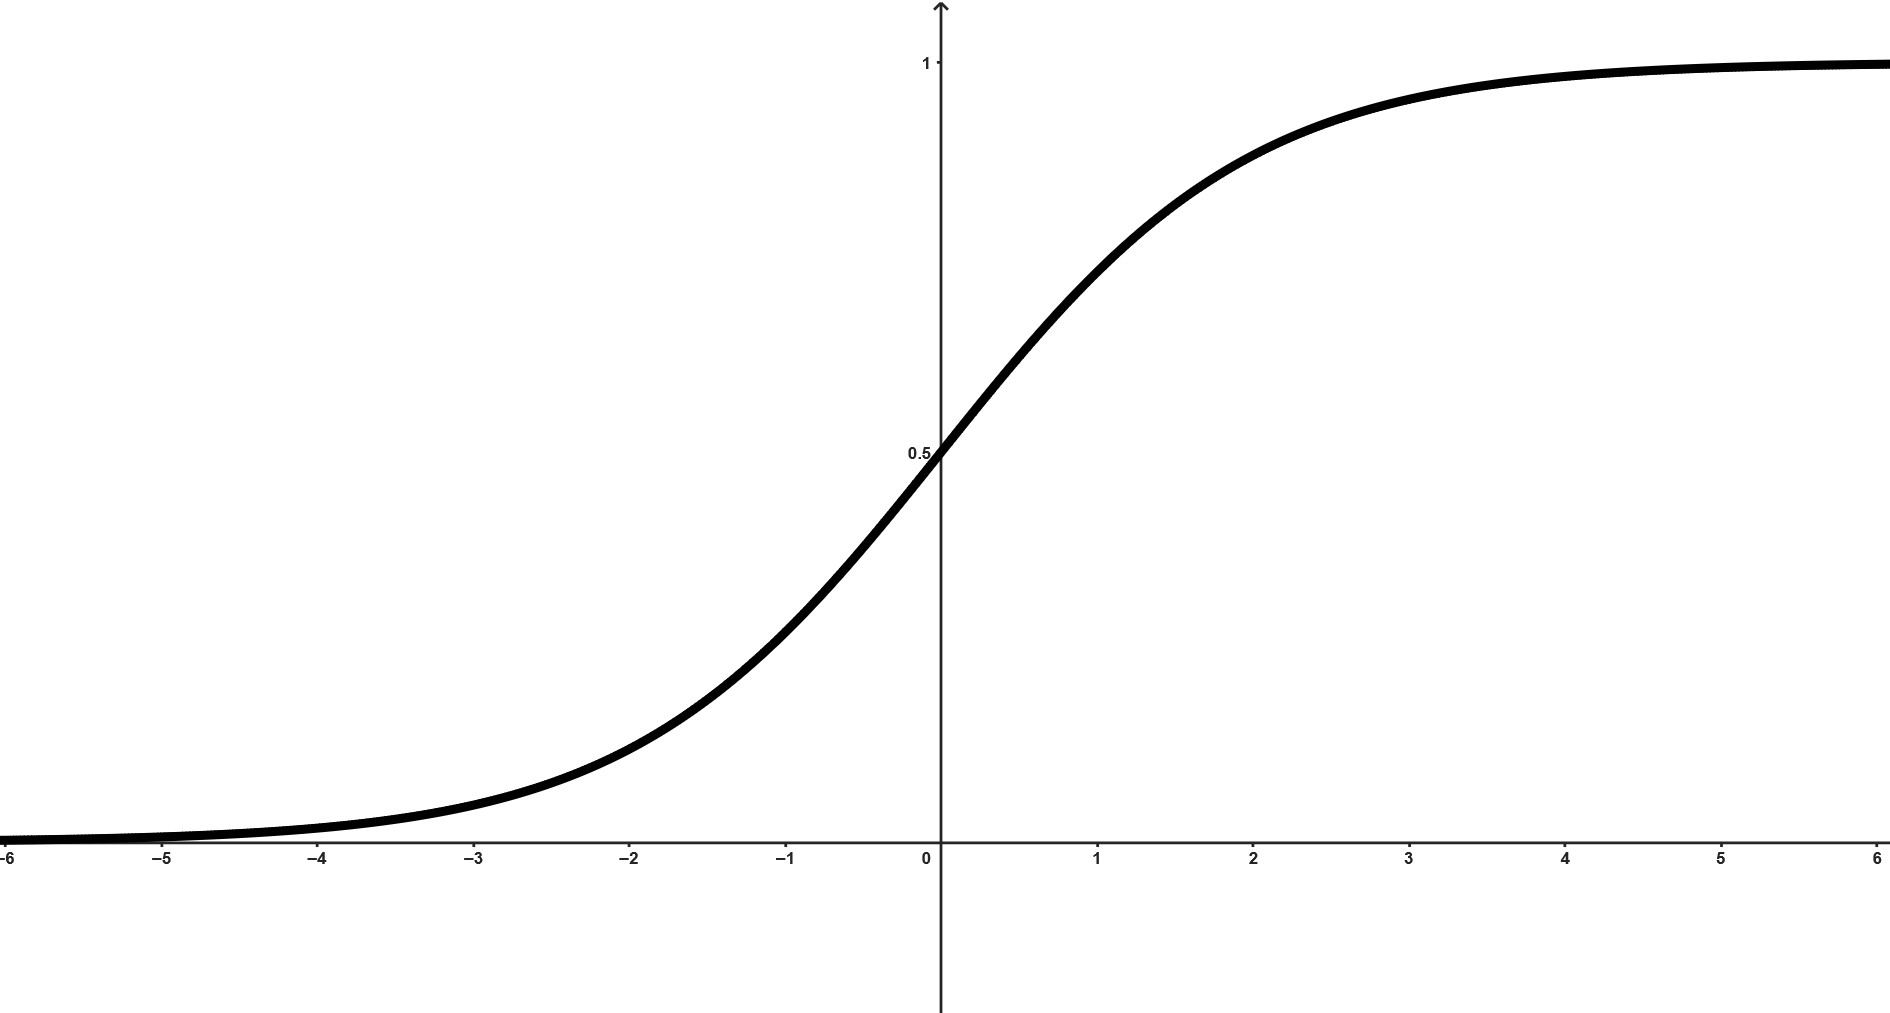
\includegraphics[width=\textwidth]{zeichnungen/sigmoid.png}
    \caption{Die Sigmoid-Funktion}\label{img:sigmoid}
\end{figure}

\begin{figure}
    \centering
    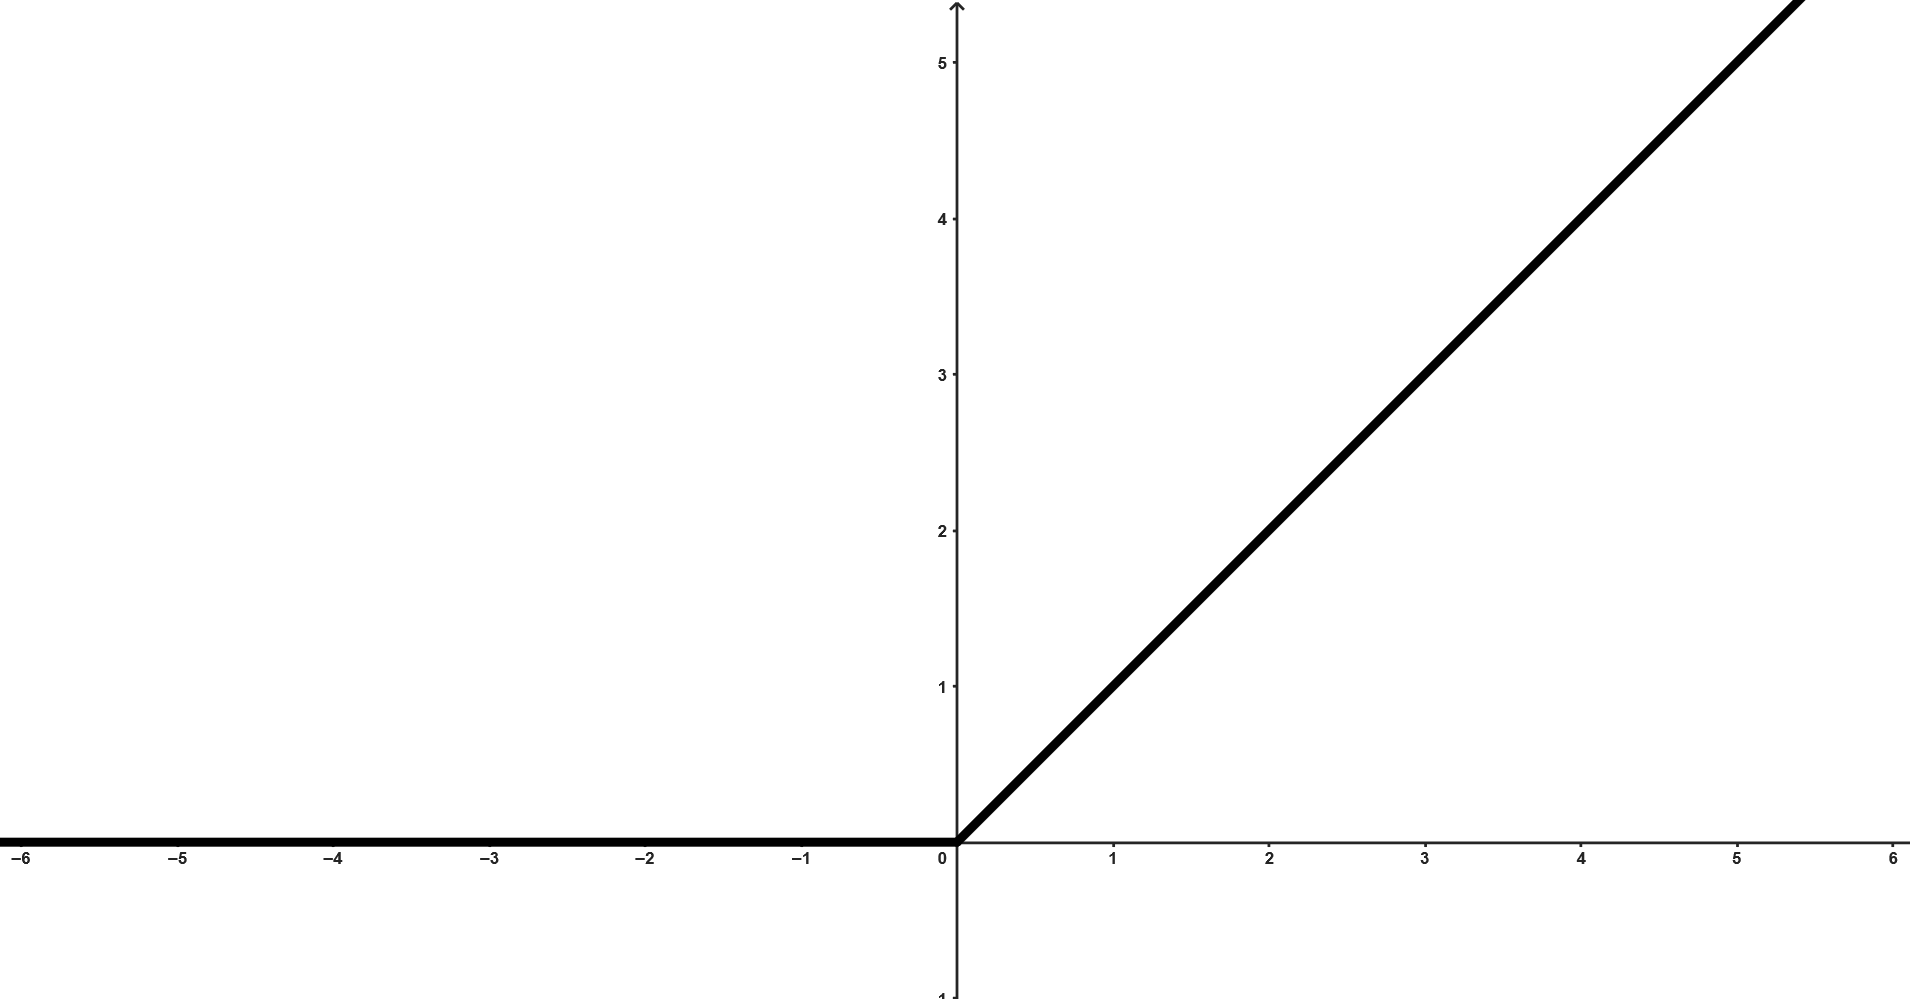
\includegraphics[width=\textwidth]{zeichnungen/relu.png}
    \caption{Die ReLU-Funktion}\label{img:relu}
\end{figure}

\begin{definition}\label{def:aktivierungsfunktion}
    Die \textbf{Aktivierungsfunktion} weißt jedem potentiellen Wert eines Neurons einen Wert in einem vorgegebenem Intervall zu.
    Sie ist nicht-linear und verhindert somit die Reduzierung eines Neuronalen Netzes auf eine lineare Funktion.
\end{definition}

Die Funktionen sind in \cref{img:sigmoid,img:relu} dargestellt.
Üblicherweise repräsentiert eine Aktivierungsfunktion eine Transformation der Eingabewerte auf einen nichtlinearen Ausgabewert zwischen 0 und 1.
Jedoch ist dies nicht zwingend notwendig, da zum Beispiel die ReLU Funktion Werte zwischen 0 und $\infty$ ausgibt, sich jedoch schneller berechnen lässt als die Sigmoid-Funktion.
Aktivierungsfunktion sind notwendig, um die Komplexität eines Neuronalen Netzes zu erhöhen und damit die Fähigkeit komplexere Probleme zu lösen, zu ermöglichen.
Ohne eine Aktivierungsfunktion würden $A_N$ Neuronen eine Linearkombination der Eingabewerte ergeben, wodurch hier nur lineare Probleme gelöst werden können.
Ein einfaches Beispiel wäre die Berechnung der XOR-Funktion.
Die XOR-Funktion verbindet zwei Eingaben und ergibt eine Ausgabe. Ist eine der beiden Eingaben 1, soll die Ausgabe ebenso 1 sein.
Andernfalls soll die Ausgabe 0 sein.
Diese einfache Funktion kann nicht ohne eine Aktivierungsfunktion gelöst werden.\\

Die Ausgabe $A_N$ sind ebenso Werte in dem Bereich der Aktivierungsfunktion und sind nicht immer repräsentativ für das Problem, das das Neuronale Netz lösen soll.
Deshalb werden diese Werte interpretiert und repräsentieren häufig einen Confidence-Score für eine bestimmte Klasse.
Ist das Neuron $A_1$ auf dem Maximalwert 1, dann ist das Netz zu \SI{100}{\percent} sicher, dass die Eingabe der Klasse 1 enspricht.
Im Bezug auf Transformer ist die Ausgabe $A_N$ ein Vektor über das gesamte Vokabular des Transformers und gibt an, in wie fern das Modell glaubt, der jeweilige Token folgt auf den Eingabetext.\\

\subsection{Training}\label{subsec:grundlagen:training}
Bevor ein Neuronales Netz korrekte Ausgaben liefern kann, muss es trainiert werden.
Trainig bedeutet das iterative Anpassen der lernbaren Parameter, um eine möglichst gute Ausgabe zu erhalten.
Eine gute Ausgabe wird durch eine Fehlerfunktion beschrieben.
Diese Fehlerfunktion gibt einen einzelnen Wert zurück, gegeben der Eingaben in das Neuronale Netz, und steht invers proportional zur richtigen Ausgabe.
Geometrisch repräsentiert eine Fehlerfunktion eine multidimensionale Fläche mit jedem lernbaren Parameter als Achse, in der das Minimum dieser Fläche ein Optimum darstellt.
Dieses Optimum ist das Ziel des Trainings.
Kleine Veränderungen in einzelnen Parametern verändern die Ausgabe der Fehlerfunktion und können somit zeigen, ob diese Veränderung zu einer Verbesserung oder Verschlechterung des Neuronalen Netzes geführt hat.
Hier existiert auch bereits die Unterscheidung zwischen einem Überwachten, Selbstüberwachten und Unüberwachten Lernverfahren.\\

\begin{definition}\label{def:ueberwachtes-lernen}
    Bei dem \textbf{Überwachten Lernen} sind während des Training sowohl die Eingabe als auch die erwartete Ausgabe bekannt.
    Die genutzte Fehlerfunktion ergibt sich aus der Differenz der erwarteten Ausgabe und der tatsächlichen Ausgabe.
\end{definition}

\begin{definition}\label{def:unueberwachtes-lernen}
    Bei dem \textbf{Unüberwachten Lernen} ist während des Training nur die Eingabe bekannt.
    Die Fehlerfunktion muss errechnet oder erschlossen werden auf Basis des Kontextes.
\end{definition}

\begin{definition}\label{def:selbstueberwachtes-lernen}
    Bei dem \textbf{selbstüberwachten Lernen} ist während des Training nur die Eingabe bekannt.
    Jedoch entspricht die Ausgabe einem Teil der Eingabe, wodurch die Fehlerfunktion errechnet werden kann.
\end{definition}

Ein Beispiel für ein Überwachtes Lernen wäre die Klassifizierung von Bildern.
Der Datensatz enthält sowohl Bilder, als auch zugehörige Klassen.
Somit ist die erwartete Ausgabe des Modells zu einem Bild exakt die Klasse.
Transformer-Modelle sind Selbstüberwachte Systeme.
Hier ergibt sich aus der Eingabe die erwartete Ausgabe, da der darauf folgende Token der Eingabe als korrekt angesehen wird.
Unüberwachtes Verfahren sind zum Beispiel Agents, welche Spiele lernen.
Hier existiert in den meisten Fällen eine Belohnungsfunktion, welche angibt, wie gut das Modell gespielt hat.
Belohnungsfunktionen können beschreiben, wie weit das Auto im Spiel gefahren ist oder wie viele Punkte gesammelt wurden.\\

\subsubsection{Backpropagation}
\begin{definition}\label{def:backpropagation}
    \textbf{Backpropagation} beschreibt den Prozess des iterativen Anpassens von Gewichten und Bias auf Basis des Gradienten einer Fehlerfunktion.
\end{definition}

Eine der wichtigsten Methoden zum iterativen Anpassen der Gewichte und Bias und damit dem Training von neuronalen Netzen ist die Fehlerrückführungsmethode (engl. Backprogatation).
Diese Gradienten-Abstiegsmethode wurde erstmalig 1986 von \citet{backpropagation} beschrieben und lässt sich im Detail in \citet{neuronale-netze} nachlesen.
Um den Rahmen dieser Arbeit nicht zu sprengen, wird hier von einer mathematischen Beschreibung abgesehen und nur die Grundidee beschrieben.\\

Die Fehlerfunktion $C$ ist eine Funktion über alle Gewichte und Bias des Neuronalen Netzes und ihrer Ausgabe.
Ihr Minimum zu finden bedeutet ein Optimum für das Modell zu finden.
Zu Beginn des Trainings werden alle Gewichte mit Zufallszahlen initialisiert.
Nun wird die Ausgabe des Modells berechnet und mit der erwarteten Ausgabe verglichen.
Die Funktion $C$ besitzt einen Gradienten $\Delta C$, welcher die Richtung des steilsten Anstiegs der Funktion beschreibt.
Möchte man die Funktion also minimieren, wird der Gradient in die entgegengesetzte Richtung angewandt.
Dieser Gradient setzt sich aus partiellen Ableitung der Fehlerfunktion über alle lernbare Parameter zusammen.\\

\paragraph{Lernrate}
\begin{definition}\label{def:lernrate}
    Die \textbf{Lernrate} entspricht der Schrittweite des Gradientenabstiegs. Höhere Lernraten führen zu schnelleren Lernprozessen, können jedoch auch zu Oszillationen führen.
    Kleinere Lernraten führen zu langsameren Lernprozessen und können möglicherweise nicht zu einem Minimum konvergieren.
\end{definition}
Den Prozess des \enquote{in Richtung des Minimum schreiten} bedeutet, die lernbaren Parameter den partiellen Ableitungen folgend anzupassen.
Die Anpassung der Parameter ist ein Hyperparameter des Trainings und wird als Lernrate bezeichnet (engl. Learning Rate).\\

\begin{definition}\label{def:hyperparameter}
    \textbf{Hyperparameter} sind Parameter, die Eigenschaften oder Techniken des Modells repräsentieren, und vor dem Training eingestellt werden.
    Sie sind nicht durch das Neuronale Netz erlernbar.
\end{definition}

Wählt man die Lernrate zu hoch, besteht die Gefahr, dass ein Minimum der Fehlerfunktion übersprungen wird und um diesen Punkt osziliert.
Wählt man die Lernrate zu niedrig, braucht das Training des Neuronalen Netzes zu lange um das Minimum zu erreichen.
In Transformern und tiefen Neuronalen Netzen ist die Lernrate nicht konstant, sondern wird über den Prozess des Trainings regelmäßig angepasst.
Sehr große Modelle besitzen oft mehrere Milliarden Parameter und benötigen daher eine sehr kleine Lernrate um nicht zu oszillieren.
Zu Beginn eines Trainings passt sich das Modell mit höhere Lernrate zu stark an kleine Änderungen an und findet ein lokales Minimum, welches weit aus über dem globalen Minimum liegt.
Daher wird eine Aufwärmphase (engl. Warmup) genutzt, um die Lernrate langsam zu erhöhen und das Modell an die Daten anzupassen.
Nach der Aufwärmphase wird die Lernrate langsam verringert, so dass anfänglich große Anpassungen der Parameter möglich sind, gegen Ende des Trainings das gefundene Minimum nur noch feinjustiert wird.\\

\paragraph{Stochastischer Gradientenabstieg}\mbox{}\\
Die Berechnung des Gradienten der Fehlerfunktion über alle lernbaren Parameter ist nur sinnvoll, wenn sie über den gesamten Datensatz berechnet wird.
Jede Eingabe des Datensatzes verändert die Ausgabe des Modells und somit auch die Fehlerfunktion.
Die Summe der Fehlerfunktionen über alle Eingaben des Datensatzes ist die Fehlerfunktion des gesamten Datensatzes.

\begin{equation}
    C = \frac{1}{n}\sum_{k=0}^{n-1}C_k\\
\end{equation}

Hierbei ist $n$ die Anzahl der Eingaben des Datensatzes und $C_k$ die Fehlerfunktion der $k$-ten Eingabe.
Die Berechnung des Gradienten über alle Eingaben des Datensatzes ist jedoch sehr rechenintensiv und wird daher durch eine Stichprobe des Datensatzes ersetzt.
Diese Stichprobe wird als Batch bezeichnet.\\

\begin{definition}\label{def:batch}
    Ein \textbf{Batch} repräsentiert eine Teilmenge an Eingaben, welche geschlossen verarbeitet werden, bevor die Gewichte und Bias angepasst werden.
\end{definition}

Die Größe des Batches ist ein weiterer Hyperparameter des Trainings.
Die Berechnung des Gradienten über einen Batch wird als Stochastischer Gradientenabstieg (engl. Stochastic Gradient Descent) bezeichnet, da die Stichprobe des Datensatzes nur eine Approximation des Gradienten ist.
Dadurch gleicht die Richtung des Gradient nur noch annäherungsweise dem tatsächlichen Gradienten, die Berechnung verläuft jedoch deutlich schneller.
Die Größe der Batches ist ein Kompromiss zwischen der Genauigkeit des Gradienten und der Geschwindigkeit der Berechnung.\\

\paragraph{Overfitting}
\begin{definition}\label{def:overfitting}
    \textbf{Overfitting} beschreibt den Prozess, bei dem ein Modell die Trainingsdaten auswendig lernt und nicht mehr in der Lage ist,
    neue Daten korrekt zu klassifizieren. Overfitting lässt sich durch einen Leistungsabfall zwischen Trainings- und Testdaten erkennen.
\end{definition}

Ein logisches Ende des Trainings ist erreicht, wenn die Fehlerfunktion sich über einen Zeitraum nicht mehr verändert und somit ein lokales Minimum gefunden wurde.
Dieses lokale Minimum ist jedoch nicht immer gewünscht.
Modelle, die den Datensatz auswendig lernen erzielen bei der Fehlerfunktion einen sehr guten Wert, der Prozess der Backprogatation wirkt fördernd.
Jedoch können diese Modelle keine neuen Daten korrekt klassifizieren und sind daher ungeeignet in der Praxis.
Diesen Prozess des Auswendiglernens wird als Overfitting bezeichnet.\\

Overfitting wird kann durch verschiedene Methoden verhindert werden.
Zur Erkennung von Overfitting wird der Datensatz in Trainings- und Testdaten aufgeteilt.
Trainiert wird nur auf den Trainingsdaten, verglichen wird jedoch mit den Testdaten.
Dadurch kann festgestellt werden, in wie fern das Modell auf Daten, die es noch nicht gesehen hat, generalisiert.
Nähert sich die Fehlerfunktion einem Minimum bei den Testdaten, kann das Training beendet werden, da weitere Anpassungen der Parameter lediglich zum Auswendiglernen des Trainigsdatensatzes führen.\\


\section{Datenverarbeitung}\label{sec:datenverarbeitung}
Um ein Modell trainieren zu können, müssen verwendeten Datensätze in eine Form verständlich für das Modell gebracht werden.
Ebenso müssen Ausgaben des Modells evaluiert werden, um die Leistungsfähigkeit des Modells zu bestimmen.\\
\begin{definition}\label{def:datenkuration}
    \textbf{Datenkuration} beschreibt den Prozess der Datenaufbereitung, um diese für die Verarbeitung durch ein Modell vorzubereiten.
\end{definition}
Die Datenkuration ist ein wichtiger Schritt dieser Arbeit und wird weiter in \cref{sec:datenkuration} genauer beschrieben.
Da Modelle nicht mit normalen Text-Dateien wie zum Beispiel Word oder PDF umgehen können, müssen diese in eine für das Modell Verständliche Form umgewandelt werden.

\subsection{Glossar der Daten}
In dieser Arbeit dreht sich vieles um Daten und deren Information und Wissen die sie enthalten.
Um diese Unterscheidung besser zu verstehen, folgt hier die Definition jener nach \citet{bb}.

\begin{definition}\label{def:wissen}
    \textbf{Wissen} sind generelle Informationen über Konzepte in einer bestimmten Domäne.
\end{definition}
Im Kontext dieser Arbeit repräsentiert Wissen Informationen aus \citet{bb}.
Diese Informationen sollen von einem Modell erlernt werden, damit das darin enthaltene Wissen wiedergeben kann.

\begin{definition}\label{def:information}
    \textbf{Informationen} sind spezifische Festlegungen über Entitäten wie zum Beispiel Fakten, Dinge, Personen, Prozesse, Ideen, Konzepte oder Ereignisse.
\end{definition}
Eine Information ist unabhängig von ihrer Darstellung und ist das grundlegende Ziel dieser Arbeit.
Informationen können unterschiedlich formuliert werden, enthalten aber gleichen Informationsgehalt.
Daher gilt wie in \cref{sec:approach:questions} beschrieben eine Antwort mit richtigen Informationen auf eine Frage unabhängig von ihrer Darstellung als richtig.

\begin{definition}\label{def:daten}
    \textbf{Daten} sind Informationen oder Wissen in einer strukturierten Form, die für die Verarbeitung, Kommunikation oder Interpretation von Menschen oder Maschinen geeignet sind.
\end{definition}
Daten werden genutzt um die Informationen und das Wissen aus \citet{bb} zu repräsentieren.
Das Modell enthält ebenso Daten, jedoch in einer für das Modell verständlichen Form.
Antworten des Modells auf Fragen sind ebenso Daten, die jedoch in einer für Menschen verständlichen Form vorliegen müssen.


\subsection{Evaluierung}
Um die Leistungsfähigkeit eines Modells zu bestimmen, müssen die Ausgaben des Modells evaluiert werden.
Diese Evaluierung ist weiter in \cref{sec:approach:comparison} beschrieben.
Zur Quantifizierung der Leistungsfähigkeit werden Metriken verwendet.
Die Berechnung dieser Metriken findet sich ebenso in \cref{sec:approach:comparison}.
Die dort genannten Metriken Micro-F1 und Macro-F1 besitzen jedoch einen grundlegenden Unterschied und werden hier genauer definiert.

\begin{definition}
    \textbf{Präzision} ist der Anteil an korrekt klassifizierten Instanzen unter allen klassifizierten Instanzen.
\end{definition}

\begin{definition}
    \textbf{Recall} ist der Anteil an korrekt klassifizierten Instanzen unter allen Instanzen.
\end{definition}
Eine Instanz beschreibt im Kontext dieser Arbeit eine Frage. Fragen können richtig beantwortet werden und gelten dann als korrekt klassifiziert.
Fragen können ebenso auch nicht beantwortet werden und gelten dann als nicht klassifiziert, im Gegenzug zu falsch beantworteten Fragen, die als falsch klassifiziert gelten.\\

\begin{definition}\label{def:micro-f1}
    Der \textbf{Micro-F1} Wert repräsentiert das harmonische Mittel aus Präzision und Recall.
    Er repräsentiert die Gesamtleistung unabhängig von der Klassenzugehörigkeit.
\end{definition}

\begin{definition}\label{def:macro-f1}
    Der \textbf{Macro-F1} Wert repräsentiert den arithmetischen Mittelwert aller F1 Werte jeder Klasse.
    Er stellt in einem nicht-balancierten Datensatz eine bessere Metrik dar, um alle Klassen gleich zu gewichten.
\end{definition}

Klassen repräsentieren Gruppen aus Instanzen. Mehrere Instanzen können zu einer Klasse gehören und werden als korrekt klassifiziert angesehen, wenn diese Klasse gewählt wurde.
Eine genauere Begründung welche Metrik in dieser Arbeit genutzt wird, findet sich unter \cref{sec:approach:comparison}.
